\documentclass{article}\usepackage[]{graphicx}\usepackage[]{xcolor}
% maxwidth is the original width if it is less than linewidth
% otherwise use linewidth (to make sure the graphics do not exceed the margin)
\makeatletter
\def\maxwidth{ %
  \ifdim\Gin@nat@width>\linewidth
    \linewidth
  \else
    \Gin@nat@width
  \fi
}
\makeatother

\definecolor{fgcolor}{rgb}{0.345, 0.345, 0.345}
\newcommand{\hlnum}[1]{\textcolor[rgb]{0.686,0.059,0.569}{#1}}%
\newcommand{\hlsng}[1]{\textcolor[rgb]{0.192,0.494,0.8}{#1}}%
\newcommand{\hlcom}[1]{\textcolor[rgb]{0.678,0.584,0.686}{\textit{#1}}}%
\newcommand{\hlopt}[1]{\textcolor[rgb]{0,0,0}{#1}}%
\newcommand{\hldef}[1]{\textcolor[rgb]{0.345,0.345,0.345}{#1}}%
\newcommand{\hlkwa}[1]{\textcolor[rgb]{0.161,0.373,0.58}{\textbf{#1}}}%
\newcommand{\hlkwb}[1]{\textcolor[rgb]{0.69,0.353,0.396}{#1}}%
\newcommand{\hlkwc}[1]{\textcolor[rgb]{0.333,0.667,0.333}{#1}}%
\newcommand{\hlkwd}[1]{\textcolor[rgb]{0.737,0.353,0.396}{\textbf{#1}}}%
\let\hlipl\hlkwb

\usepackage{framed}
\makeatletter
\newenvironment{kframe}{%
 \def\at@end@of@kframe{}%
 \ifinner\ifhmode%
  \def\at@end@of@kframe{\end{minipage}}%
  \begin{minipage}{\columnwidth}%
 \fi\fi%
 \def\FrameCommand##1{\hskip\@totalleftmargin \hskip-\fboxsep
 \colorbox{shadecolor}{##1}\hskip-\fboxsep
     % There is no \\@totalrightmargin, so:
     \hskip-\linewidth \hskip-\@totalleftmargin \hskip\columnwidth}%
 \MakeFramed {\advance\hsize-\width
   \@totalleftmargin\z@ \linewidth\hsize
   \@setminipage}}%
 {\par\unskip\endMakeFramed%
 \at@end@of@kframe}
\makeatother

\definecolor{shadecolor}{rgb}{.97, .97, .97}
\definecolor{messagecolor}{rgb}{0, 0, 0}
\definecolor{warningcolor}{rgb}{1, 0, 1}
\definecolor{errorcolor}{rgb}{1, 0, 0}
\newenvironment{knitrout}{}{} % an empty environment to be redefined in TeX

\usepackage{alltt}
\usepackage[margin=1.0in]{geometry} % To set margins
\usepackage{amsmath}  % This allows me to use the align functionality.
                      % If you find yourself trying to replicate
                      % something you found online, ensure you're
                      % loading the necessary packages!
\usepackage{amsfonts} % Math font
\usepackage{fancyvrb}
\usepackage{hyperref} % For including hyperlinks
\usepackage[shortlabels]{enumitem}% For enumerated lists with labels specified
                                  % We had to run tlmgr_install("enumitem") in R
\usepackage{float}    % For telling R where to put a table/figure
\usepackage{natbib}        %For the bibliography
\bibliographystyle{apalike}%For the bibliography
\IfFileExists{upquote.sty}{\usepackage{upquote}}{}
\begin{document}


\begin{enumerate}
%%%%%%%%%%%%%%%%%%%%%%%%%%%%%%%%%%%%%%%%%%%%%%%%%%%%%%%%%%%%%%%%%%%%%%%%%%%%%%%%
%%%%%%%%%%%%%%%%%%%%%%%%%%%%%%%%%%%%%%%%%%%%%%%%%%%%%%%%%%%%%%%%%%%%%%%%%%%%%%%%
% Question 1
%%%%%%%%%%%%%%%%%%%%%%%%%%%%%%%%%%%%%%%%%%%%%%%%%%%%%%%%%%%%%%%%%%%%%%%%%%%%%%%%
%%%%%%%%%%%%%%%%%%%%%%%%%%%%%%%%%%%%%%%%%%%%%%%%%%%%%%%%%%%%%%%%%%%%%%%%%%%%%%%%
\item When conducting the work of Lab 11, we conducted the test that uses the
Central Limit Theorem even though the sample size was ``small" (i.e., $n<30$).
It turns out, that how ``far off" the $t$-test is can be computed using
a first-order Edgeworth approximation for the error. Below, we will do this 
for the the further observations.
\begin{enumerate}
  \item \cite{Boos00} note that 
  \begin{align*}
    P(T \leq t) \approx F_Z(t) + \underbrace{\frac{\text{skew}}{\sqrt{n}} \frac{(2t^2+1)}{6} f_Z(t)}_{\textrm{error}},
  \end{align*}
  where $f_Z(\cdot)$ and $F_Z(\cdot)$ are the Gaussian PDF and CDF and skew is the
  skewness of the data. What is the potential error in the computation of the 
  $p$-value when testing $H_0: \mu_X=0; H_a: \mu_X<0$ using the zebra finch further data? 
\begin{knitrout}
\definecolor{shadecolor}{rgb}{0.969, 0.969, 0.969}\color{fgcolor}\begin{kframe}
\begin{alltt}
\hlkwd{library}\hldef{(tidyverse)}
\hlkwd{library}\hldef{(xtable)}
\hlkwd{library}\hldef{(VGAM)}
\hlkwd{library}\hldef{(e1071)}
\hlkwd{library}\hldef{(pwr)}
\hlkwd{library}\hldef{(effectsize)}
\hlcom{### Part A ### -> using further observations}
\hldef{dat.finches} \hlkwb{<-} \hlkwd{read.csv}\hldef{(}\hlsng{"zebrafinches.csv"}\hldef{)}

\hldef{further} \hlkwb{<-} \hldef{dat.finches}\hlopt{$}\hldef{further}
\hldef{mu0} \hlkwb{<-} \hlnum{0}
\hldef{t.further} \hlkwb{<-} \hlkwd{t.test}\hldef{(further,}
                    \hlkwc{mu} \hldef{= mu0,}
                    \hlkwc{alternative} \hldef{=} \hlsng{"less"}\hldef{)}
\hldef{t.stat.further} \hlkwb{<-} \hldef{t.further}\hlopt{$}\hldef{statistic}
\hldef{n} \hlkwb{<-} \hlkwd{length}\hldef{(further)}
\hldef{skewness} \hlkwb{<-} \hlkwd{skewness}\hldef{(further)}
\hldef{fz} \hlkwb{<-} \hlkwd{dnorm}\hldef{(t.stat.further)}
\hldef{Fz} \hlkwb{<-} \hlkwd{pnorm}\hldef{(t.stat.further)}

\hldef{(edgeworth.approx.error} \hlkwb{<-} \hldef{(skewness}\hlopt{/}\hlkwd{sqrt}\hldef{(n))} \hlopt{*}
    \hldef{(((}\hlnum{2}\hlopt{*}\hldef{(t.stat.further)}\hlopt{^}\hlnum{2} \hlopt{+} \hlnum{1}\hldef{)}\hlopt{/}\hlnum{6}\hldef{)}\hlopt{*}\hldef{(fz)))}
\end{alltt}
\begin{verbatim}
##             t 
## -1.226006e-13
\end{verbatim}
\begin{alltt}
\hlcom{# Potential Error in the computation of the p-value is -1.226006e-13.}
\hldef{probability} \hlkwb{<-} \hldef{Fz} \hlopt{+} \hldef{edgeworth.approx.error}
\end{alltt}
\end{kframe}
\end{knitrout}
We found the Edgeworth approximation error to be -1.226006e-13 which is very close to 0. This means that the t-test is not "far-off" due to the potential error in the computation of the p-value when testing the hypotheses for the further data being so low. 
  \item Compute the error for $t$ statistics from -10 to 10 and plot a line
  that shows the error across $t$. Continue to use the skewness and 
  the sample size for the zebra finch further data.
\begin{knitrout}
\definecolor{shadecolor}{rgb}{0.969, 0.969, 0.969}\color{fgcolor}\begin{kframe}
\begin{alltt}
\hlcom{### Part B ###}
\hldef{t.values} \hlkwb{<-} \hlkwd{seq}\hldef{(}\hlopt{-}\hlnum{10}\hldef{,}\hlnum{10}\hldef{,} \hlkwc{length} \hldef{=} \hlnum{1000}\hldef{)}
\hldef{fz2} \hlkwb{<-} \hlkwd{dnorm}\hldef{(t.values)}

\hldef{error.vals} \hlkwb{<-} \hldef{(skewness}\hlopt{/}\hlkwd{sqrt}\hldef{(n))} \hlopt{*} \hldef{(((}\hlnum{2}\hlopt{*}\hldef{(t.values)}\hlopt{^}\hlnum{2} \hlopt{+} \hlnum{1}\hldef{)}\hlopt{/}\hlnum{6}\hldef{)}\hlopt{*}\hldef{(fz2))}

\hldef{error.tvals} \hlkwb{<-} \hlkwd{tibble}\hldef{(}
  \hlkwc{t} \hldef{= t.values,}
  \hlkwc{error} \hldef{= error.vals}
\hldef{)}
\hldef{(}\hlkwd{summary}\hldef{(error.tvals))}
\end{alltt}
\begin{verbatim}
##        t           error           
##  Min.   :-10   Min.   :-2.602e-02  
##  1st Qu.: -5   1st Qu.:-8.061e-03  
##  Median :  0   Median :-2.560e-06  
##  Mean   :  0   Mean   :-5.172e-03  
##  3rd Qu.:  5   3rd Qu.: 0.000e+00  
##  Max.   : 10   Max.   : 0.000e+00
\end{verbatim}
\begin{alltt}
\hldef{error.t.plot} \hlkwb{<-} \hlkwd{ggplot}\hldef{()}\hlopt{+}
  \hlkwd{geom_line}\hldef{(}\hlkwc{data} \hldef{= error.tvals,}
            \hlkwd{aes}\hldef{(}\hlkwc{x} \hldef{= t,} \hlkwc{y} \hldef{= error),}
            \hlkwc{color} \hldef{=} \hlsng{"lightblue"}\hldef{)}\hlopt{+}
  \hlkwd{theme_bw}\hldef{()}\hlopt{+}
  \hlkwd{labs}\hldef{(}\hlkwc{title} \hldef{=} \hlsng{"Edgeworth Approximation Error"}\hldef{,}
       \hlkwc{x} \hldef{=} \hlsng{"T Values (-10,10)"}\hldef{,}
       \hlkwc{y} \hldef{=} \hlsng{"Error"}\hldef{)}
\end{alltt}
\end{kframe}
\end{knitrout}
\begin{figure}[H]
\begin{center}
\begin{knitrout}
\definecolor{shadecolor}{rgb}{0.969, 0.969, 0.969}\color{fgcolor}

{\centering 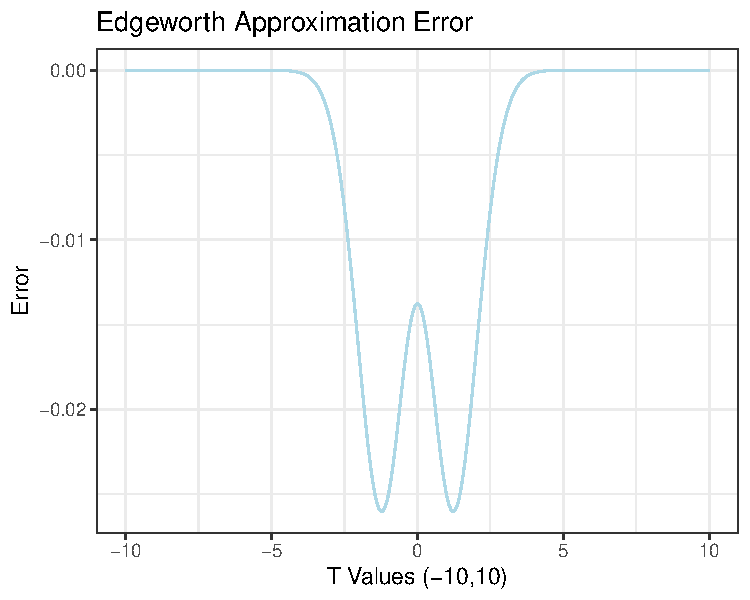
\includegraphics[width=\maxwidth]{figure/unnamed-chunk-3-1} 

}


\end{knitrout}
\caption{Edgeworth Approximation Error Across t values}
\label{plot1} 
\end{center}
\end{figure}
For the error across the t-values from -10 to 10, we can see that the maximum error is essentially 0 with the median being around -2.56e-06 at around t=0. 
  \item Suppose we wanted to have a tail probability within 10\% of the desired
  $\alpha=0.05$. Recall we did a left-tailed test using the further data.
  How large of a sample size would we need? That is, we need
  to solve the error formula equal to 10\% of the desired left-tail probability:
  \[0.10 \alpha  \stackrel{set}{=} \underbrace{\frac{\text{skew}}{\sqrt{n}} \frac{(2t^2+1)}{6} f_Z(t)}_{\textrm{error}},\]
  which yields
  \[ n = \left(\frac{\text{skew}}{6(0.10\alpha)} (2t^2 + 1) f_Z(t)\right)^2.\]
\begin{knitrout}
\definecolor{shadecolor}{rgb}{0.969, 0.969, 0.969}\color{fgcolor}\begin{kframe}
\begin{alltt}
\hlcom{### Part C ### - error in the rejection region}
\hldef{skewness} \hlkwb{<-} \hlkwd{skewness}\hldef{(further)}
\hldef{tval} \hlkwb{<-} \hlkwd{qnorm}\hldef{(}\hlnum{0.05}\hldef{)}
\hldef{fz3} \hlkwb{<-} \hlkwd{dnorm}\hldef{(tval)}

\hldef{(min.n} \hlkwb{<-} \hldef{((skewness}\hlopt{/}\hldef{(}\hlnum{6}\hlopt{*}\hldef{(}\hlnum{0.10}\hlopt{*}\hlnum{0.05}\hldef{)))} \hlopt{*} \hldef{(}\hlnum{2}\hlopt{*}\hldef{tval}\hlopt{^}\hlnum{2} \hlopt{+} \hlnum{1}\hldef{)} \hlopt{*}\hldef{fz3)}\hlopt{^}\hlnum{2}\hldef{)}
\end{alltt}
\begin{verbatim}
## [1] 520.8876
\end{verbatim}
\end{kframe}
\end{knitrout}
We would need a sample size of n = 520.8876 for a left-tailed test. This is much larger than the current n.  
  
\end{enumerate}
%%%%%%%%%%%%%%%%%%%%%%%%%%%%%%%%%%%%%%%%%%%%%%%%%%%%%%%%%%%%%%%%%%%%%%%%%%%%%%%%
%%%%%%%%%%%%%%%%%%%%%%%%%%%%%%%%%%%%%%%%%%%%%%%%%%%%%%%%%%%%%%%%%%%%%%%%%%%%%%%%
% Question 2
%%%%%%%%%%%%%%%%%%%%%%%%%%%%%%%%%%%%%%%%%%%%%%%%%%%%%%%%%%%%%%%%%%%%%%%%%%%%%%%%
%%%%%%%%%%%%%%%%%%%%%%%%%%%%%%%%%%%%%%%%%%%%%%%%%%%%%%%%%%%%%%%%%%%%%%%%%%%%%%%%
\item Complete the following steps to revisit the analyses from lab 11 using the
bootstrap procedure.
\begin{enumerate}
\item Now, consider the zebra finch data. We do not know the generating distributions
for the closer, further, and difference data, so perform resampling to approximate the 
sampling distribution of the $T$ statistic:
  \[T = \frac{\bar{x}_r - 0}{s/\sqrt{n}},\]
  where $\bar{x}_r$ is the mean computed on the r$^{th}$ resample and $s$ is the
  sample standard deviation from the original samples. At the end, create an
  object called \texttt{resamples.null.closer}, for example, and store the 
  resamples shifted to ensure they are consistent with the null hypotheses at the average 
  (i.e., here ensure the shifted resamples are 0 on average, corresponding
  to $t=0$, for each case). 
\begin{knitrout}
\definecolor{shadecolor}{rgb}{0.969, 0.969, 0.969}\color{fgcolor}\begin{kframe}
\begin{alltt}
\hlkwd{library}\hldef{(boot)}
\hlcom{### Part A ###}

\hlcom{# Closer Resamples}
\hldef{R} \hlkwb{<-} \hlnum{10000}
\hldef{s.closer} \hlkwb{<-} \hlkwd{sd}\hldef{(dat.finches}\hlopt{$}\hldef{closer)}
\hldef{n.closer} \hlkwb{<-} \hlkwd{length}\hldef{(dat.finches}\hlopt{$}\hldef{closer)}
\hldef{resamples.closer} \hlkwb{<-}  \hlkwd{tibble}\hldef{(}\hlkwc{tstat}\hldef{=}\hlkwd{rep}\hldef{(}\hlnum{NA}\hldef{, R),}
                            \hlkwc{xbar}\hldef{=}\hlkwd{rep}\hldef{(}\hlnum{NA}\hldef{, R))}
\hlkwa{for}\hldef{(i} \hlkwa{in} \hlnum{1}\hlopt{:}\hldef{R)\{}
  \hldef{curr.resample} \hlkwb{<-} \hlkwd{sample}\hldef{(}\hlkwc{x} \hldef{= dat.finches}\hlopt{$}\hldef{closer,}
                          \hlkwc{size} \hldef{= n.closer,}
                          \hlkwc{replace} \hldef{= T)}
  \hldef{resamples.closer}\hlopt{$}\hldef{tstat[i]} \hlkwb{<-} \hldef{(}\hlkwd{mean}\hldef{(curr.resample)}\hlopt{-}\hlnum{0}\hldef{)}\hlopt{/}\hldef{(s.closer}\hlopt{/}\hlkwd{sqrt}\hldef{(n.closer))}
  \hldef{resamples.closer}\hlopt{$}\hldef{xbar[i]} \hlkwb{<-} \hlkwd{mean}\hldef{(curr.resample)}
\hldef{\}}
\hlcom{# shift so H0 is true}
\hldef{delta.closer} \hlkwb{<-} \hlkwd{mean}\hldef{(resamples.closer}\hlopt{$}\hldef{tstat)} \hlopt{-} \hlnum{0} \hlcom{# null mu0 = 0}

\hldef{resamples.null.closer} \hlkwb{<-} \hldef{resamples.closer |>}
  \hlkwd{mutate}\hldef{(}\hlkwc{tstat.shifted} \hldef{= tstat} \hlopt{-} \hldef{delta.closer)}

\hldef{(}\hlkwd{mean}\hldef{(resamples.null.closer}\hlopt{$}\hldef{tstat.shifted))}
\end{alltt}
\begin{verbatim}
## [1] -1.568523e-16
\end{verbatim}
\begin{alltt}
\hlcom{# Further Resamples}
\hldef{R} \hlkwb{<-} \hlnum{10000}
\hldef{s.further} \hlkwb{<-} \hlkwd{sd}\hldef{(dat.finches}\hlopt{$}\hldef{further)}
\hldef{n.further} \hlkwb{<-} \hlkwd{length}\hldef{(dat.finches}\hlopt{$}\hldef{further)}
\hldef{resamples.further} \hlkwb{<-} \hlkwd{tibble}\hldef{(}\hlkwc{tstat}\hldef{=}\hlkwd{rep}\hldef{(}\hlnum{NA}\hldef{, R),}
                            \hlkwc{xbar}\hldef{=}\hlkwd{rep}\hldef{(}\hlnum{NA}\hldef{, R))}
\hlkwa{for}\hldef{(i} \hlkwa{in} \hlnum{1}\hlopt{:}\hldef{R)\{}
  \hldef{curr.resample} \hlkwb{<-} \hlkwd{sample}\hldef{(}\hlkwc{x} \hldef{= dat.finches}\hlopt{$}\hldef{further,}
                          \hlkwc{size} \hldef{= n.further,}
                          \hlkwc{replace} \hldef{= T)}
  \hldef{resamples.further}\hlopt{$}\hldef{tstat[i]} \hlkwb{<-} \hldef{(}\hlkwd{mean}\hldef{(curr.resample)}\hlopt{-}\hlnum{0}\hldef{)}\hlopt{/}\hldef{(s.further}\hlopt{/}\hlkwd{sqrt}\hldef{(n.further))}
  \hldef{resamples.further}\hlopt{$}\hldef{xbar[i]} \hlkwb{<-} \hlkwd{mean}\hldef{(curr.resample)}
\hldef{\}}
\hlcom{# shift so H0 is true}
\hldef{delta.further} \hlkwb{<-} \hlkwd{mean}\hldef{(resamples.further}\hlopt{$}\hldef{tstat)} \hlopt{-} \hlnum{0} \hlcom{# null mu0 = 0}
\hldef{resamples.null.further} \hlkwb{<-} \hldef{resamples.further |>}
  \hlkwd{mutate}\hldef{(}\hlkwc{tstat.shifted} \hldef{= tstat} \hlopt{-} \hldef{delta.further)}

\hldef{(}\hlkwd{mean}\hldef{(resamples.null.further}\hlopt{$}\hldef{tstat.shifted))}
\end{alltt}
\begin{verbatim}
## [1] 6.76903e-17
\end{verbatim}
\begin{alltt}
\hlcom{# Difference Resamples}
\hldef{R} \hlkwb{<-} \hlnum{10000}
\hldef{s.diff} \hlkwb{<-} \hlkwd{sd}\hldef{(dat.finches}\hlopt{$}\hldef{diff)}
\hldef{n.diff} \hlkwb{<-} \hlkwd{length}\hldef{(dat.finches}\hlopt{$}\hldef{diff)}
\hldef{resamples.diff} \hlkwb{<-}  \hlkwd{tibble}\hldef{(}\hlkwc{tstat}\hldef{=}\hlkwd{rep}\hldef{(}\hlnum{NA}\hldef{, R),}
                          \hlkwc{xbar}\hldef{=}\hlkwd{rep}\hldef{(}\hlnum{NA}\hldef{, R))}
\hlkwa{for}\hldef{(i} \hlkwa{in} \hlnum{1}\hlopt{:}\hldef{R)\{}
  \hldef{curr.resample} \hlkwb{<-} \hlkwd{sample}\hldef{(}\hlkwc{x} \hldef{= dat.finches}\hlopt{$}\hldef{diff,}
                          \hlkwc{size} \hldef{= n.diff,}
                          \hlkwc{replace} \hldef{= T)}
  \hldef{resamples.diff}\hlopt{$}\hldef{tstat[i]} \hlkwb{<-} \hldef{(}\hlkwd{mean}\hldef{(curr.resample)}\hlopt{-}\hlnum{0}\hldef{)}\hlopt{/}\hldef{(s.diff}\hlopt{/}\hlkwd{sqrt}\hldef{(n.diff))}
  \hldef{resamples.diff}\hlopt{$}\hldef{xbar[i]} \hlkwb{<-} \hlkwd{mean}\hldef{(curr.resample)}
\hldef{\}}
\hlcom{# shift so H0 is true}
\hldef{delta.diff} \hlkwb{<-} \hlkwd{mean}\hldef{(resamples.diff}\hlopt{$}\hldef{tstat)} \hlopt{-} \hlnum{0} \hlcom{# null mu0 = 0}
\hldef{resamples.null.diff} \hlkwb{<-} \hldef{resamples.diff |>}
  \hlkwd{mutate}\hldef{(}\hlkwc{tstat.shifted} \hldef{= tstat} \hlopt{-} \hldef{delta.diff)}

\hldef{(}\hlkwd{mean}\hldef{(resamples.null.diff}\hlopt{$}\hldef{tstat.shifted))}
\end{alltt}
\begin{verbatim}
## [1] -3.604228e-16
\end{verbatim}
\end{kframe}
\end{knitrout}
We were asked to preform resampling across the closer, further, and difference data because we do not know the generating distributions for them. We use resampling to approximate the sampling distribution of the T statistic. For all three data sets, the shifted resamples are close to 0 on average which corresponds to t = 0 for each case. This ensures that the resamples shifted are consistent with the null hypothesis at the average.   
  \item Compute the bootstrap $p$-value for each test using the shifted resamples. 
  How do these compare to the $t$-test $p$-values?
\begin{knitrout}
\definecolor{shadecolor}{rgb}{0.969, 0.969, 0.969}\color{fgcolor}\begin{kframe}
\begin{alltt}
\hlcom{################# Part B ###################}
\hlcom{## Closer ##}
\hlcom{# Bootstrap P-Value}
\hldef{p.boot.closer} \hlkwb{<-} \hlkwd{mean}\hldef{(resamples.null.closer}\hlopt{$}\hldef{tstat.shifted} \hlopt{>=} \hldef{delta.closer)}
\hlcom{# T-Test P-Value}
\hldef{p.t.closer} \hlkwb{<-} \hlkwd{t.test}\hldef{(dat.finches}\hlopt{$}\hldef{closer,}
                     \hlkwc{mu} \hldef{=} \hlnum{0}\hldef{,}
                     \hlkwc{alternative} \hldef{=} \hlsng{"greater"}\hldef{)}
\hldef{p.t.closer} \hlkwb{<-} \hldef{p.t.closer}\hlopt{$}\hldef{p.value}

\hlcom{## Further ##}
\hlcom{# Bootstrap P-Value}
\hldef{p.boot.further} \hlkwb{<-} \hlkwd{mean}\hldef{(resamples.null.further}\hlopt{$}\hldef{tstat.shifted} \hlopt{<=} \hldef{delta.further)}
\hlcom{# T-Test P-Value}
\hldef{p.t.further} \hlkwb{<-} \hlkwd{t.test}\hldef{(dat.finches}\hlopt{$}\hldef{further,}
                      \hlkwc{mu} \hldef{=} \hlnum{0}\hldef{,}
                      \hlkwc{alternative} \hldef{=} \hlsng{"less"}\hldef{)}
\hldef{p.t.further} \hlkwb{<-} \hldef{p.t.further}\hlopt{$}\hldef{p.value}

\hlcom{## Difference ##}
\hlcom{# Bootstrap P-Value}
\hldef{low} \hlkwb{<-} \hlnum{0} \hlopt{-} \hldef{delta.diff}
\hldef{high} \hlkwb{<-} \hlnum{0} \hlopt{+} \hldef{delta.diff}
\hldef{p.low} \hlkwb{<-} \hlkwd{mean}\hldef{(resamples.null.diff}\hlopt{$}\hldef{tstat.shifted} \hlopt{<=} \hldef{low)}
\hldef{p.high} \hlkwb{<-} \hlkwd{mean}\hldef{(resamples.null.diff}\hlopt{$}\hldef{tstat.shifted} \hlopt{>=} \hldef{high)}
\hldef{p.boot.diff} \hlkwb{<-} \hldef{p.low} \hlopt{+} \hldef{p.high}
\hlcom{# T-Test P-Value}
\hldef{p.t.diff} \hlkwb{<-} \hlkwd{t.test}\hldef{(dat.finches}\hlopt{$}\hldef{diff,}
                   \hlkwc{mu} \hldef{=} \hlnum{0}\hldef{,}
                   \hlkwc{alternative} \hldef{=} \hlsng{"two.sided"}\hldef{)}
\hldef{p.t.diff} \hlkwb{<-} \hldef{p.t.diff}\hlopt{$}\hldef{p.value}

\hldef{comparison.pvals} \hlkwb{<-} \hlkwd{tibble}\hldef{(}
  \hlkwc{Data} \hldef{=} \hlkwd{c}\hldef{(}\hlsng{"Closer"}\hldef{,} \hlsng{"Further"}\hldef{,} \hlsng{"Difference"}\hldef{),}
  \hlkwc{`Bootstrap P-value`} \hldef{=} \hlkwd{c}\hldef{(p.boot.closer,}
                          \hldef{p.boot.further,}
                          \hldef{p.boot.diff),}
  \hlkwc{`T-Test P-value`} \hldef{=} \hlkwd{c}\hldef{(p.t.closer,}
                       \hldef{p.t.further,}
                       \hldef{p.t.diff)}
\hldef{)}
\hldef{comparison.pvals.1} \hlkwb{<-} \hlkwd{xtable}\hldef{(comparison.pvals,}
       \hlkwc{caption} \hldef{=} \hlsng{"Comparing Bootstrap p-values to t-test p-values"}\hldef{,}
       \hlkwc{label} \hldef{=} \hlsng{"tab:bootpcomp"}\hldef{)}
\end{alltt}
\end{kframe}
\end{knitrout}
% latex table generated in R 4.4.2 by xtable 1.8-4 package
% Thu May  1 15:35:00 2025
\begin{table}[H]
\centering
\begingroup\small
\begin{tabular}{lrr}
  \hline
Data & Bootstrap P-value & T-Test P-value \\ 
  \hline
Closer & 0.00 & 0.00 \\ 
  Further & 0.00 & 0.00 \\ 
  Difference & 0.00 & 0.00 \\ 
   \hline
\end{tabular}
\endgroup
\caption{Comparing Bootstrap p-values to t-test p-values} 
\label{tab:bootpcomp}
\end{table}

The table above shows the comparison of the bootstrap p-values versus the t-test p-values. For all three cases, the bootstrap test shows p-values of 0 and the t-test shows similar (essentially 0).
    \item What is the 5$^{th}$ percentile of the shifted resamples under the null hypothesis? 
  Note this value approximates $t_{0.05, n-1}$. Compare these values in each case.
\begin{knitrout}
\definecolor{shadecolor}{rgb}{0.969, 0.969, 0.969}\color{fgcolor}\begin{kframe}
\begin{alltt}
\hlcom{################# Part C ###################}
\hlcom{# Want to use shifted t stat for the p-value}
\hlcom{#Closer}
\hldef{percentile.boot.closer} \hlkwb{<-} \hlkwd{quantile}\hldef{(resamples.null.closer}\hlopt{$}\hldef{tstat.shifted,} \hlnum{0.05}\hldef{)}
\hldef{percentile.t.closer} \hlkwb{<-} \hlkwd{qt}\hldef{(}\hlnum{0.05}\hldef{,} \hlkwc{df} \hldef{= n.closer} \hlopt{-}\hlnum{1}\hldef{)}

\hlcom{#Further}
\hldef{percentile.boot.further} \hlkwb{<-} \hlkwd{quantile}\hldef{(resamples.null.further}\hlopt{$}\hldef{tstat.shifted,} \hlnum{0.05}\hldef{)}
\hldef{percentile.t.further} \hlkwb{<-} \hlkwd{qt}\hldef{(}\hlnum{0.05}\hldef{,} \hlkwc{df} \hldef{= n.further} \hlopt{-}\hlnum{1}\hldef{)}

\hlcom{#Difference}
\hldef{percentile.boot.diff} \hlkwb{<-} \hlkwd{quantile}\hldef{(resamples.null.diff}\hlopt{$}\hldef{tstat.shifted,} \hlnum{0.05}\hldef{)}
\hldef{percentile.t.diff} \hlkwb{<-} \hlkwd{qt}\hldef{(}\hlnum{0.05}\hldef{,} \hlkwc{df} \hldef{= n.diff} \hlopt{-}\hlnum{1}\hldef{)}

\hldef{comparison.percentile} \hlkwb{<-} \hlkwd{tibble}\hldef{(}
  \hlkwc{Data} \hldef{=} \hlkwd{c}\hldef{(}\hlsng{"Closer"}\hldef{,} \hlsng{"Further"}\hldef{,} \hlsng{"Difference"}\hldef{),}
  \hlkwc{`Bootstrap Percentile`} \hldef{=} \hlkwd{c}\hldef{(percentile.boot.closer,}
                             \hldef{percentile.boot.further,}
                             \hldef{percentile.boot.diff),}
  \hlkwc{`T-Test Percentile`} \hldef{=} \hlkwd{c}\hldef{(percentile.t.closer,}
                          \hldef{percentile.t.further,}
                          \hldef{percentile.t.diff)}
\hldef{)}
\hldef{comparison.percent.1} \hlkwb{<-} \hlkwd{xtable}\hldef{(comparison.percentile,}
       \hlkwc{caption} \hldef{=} \hlsng{"Comparing Bootstrap percentiles to t-test percentiles"}\hldef{,}
       \hlkwc{label} \hldef{=} \hlsng{"tab:bootperccomp"}\hldef{)}
\end{alltt}
\end{kframe}
\end{knitrout}
% latex table generated in R 4.4.2 by xtable 1.8-4 package
% Thu May  1 15:35:00 2025
\begin{table}[H]
\centering
\begingroup\small
\begin{tabular}{lrr}
  \hline
Data & Bootstrap Percentile & T-Test Percentile \\ 
  \hline
Closer & -1.59 & -1.71 \\ 
  Further & -1.70 & -1.71 \\ 
  Difference & -1.58 & -1.71 \\ 
   \hline
\end{tabular}
\endgroup
\caption{Comparing Bootstrap percentiles to t-test percentiles} 
\label{tab:bootperccomp}
\end{table}

The 5th percentile of the shifted resamples under the null hypothesis are: closer case = -1.59, further case: -1.69, and difference case = -1.54. In comparison to the t-test 5th percentile which is -1.71 for all three cases, they are very similar with small variations due to sampling variability. 
  \item Compute the bootstrap confidence intervals using the resamples. How do these 
  compare to the $t$-test confidence intervals?
\begin{knitrout}
\definecolor{shadecolor}{rgb}{0.969, 0.969, 0.969}\color{fgcolor}\begin{kframe}
\begin{alltt}
\hlcom{# Confidence Interval}
\hlcom{### use resamples for boot -- need this for x bar (floruorences)}
\hlcom{# want to use resample x bars (not shifted) for the confidence interval}
\hlcom{# Closer}
\hldef{(CI.boot.closer} \hlkwb{<-} \hlkwd{quantile}\hldef{(resamples.null.closer}\hlopt{$}\hldef{xbar,} \hlkwd{c}\hldef{(}\hlnum{0.025}\hldef{,} \hlnum{0.975}\hldef{)))}
\end{alltt}
\begin{verbatim}
##      2.5%     97.5% 
## 0.1210889 0.1922583
\end{verbatim}
\begin{alltt}
\hldef{CI.t.closer} \hlkwb{<-} \hlkwd{t.test}\hldef{(}\hlkwc{x}\hldef{=dat.finches}\hlopt{$}\hldef{closer,} \hlkwc{mu} \hldef{=} \hlnum{0}\hldef{,} \hlkwc{conf.level} \hldef{=} \hlnum{0.95}\hldef{,} \hlkwc{alternative} \hldef{=} \hlsng{"two.sided"}\hldef{)}
\hldef{(CI.t.closer} \hlkwb{<-} \hldef{CI.t.closer}\hlopt{$}\hldef{conf.int)}
\end{alltt}
\begin{verbatim}
## [1] 0.1173875 0.1950586
## attr(,"conf.level")
## [1] 0.95
\end{verbatim}
\begin{alltt}
\hlcom{# Further}
\hldef{(CI.boot.further} \hlkwb{<-} \hlkwd{quantile}\hldef{(resamples.null.further}\hlopt{$}\hldef{xbar,} \hlkwd{c}\hldef{(}\hlnum{0.025}\hldef{,} \hlnum{0.975}\hldef{)))}
\end{alltt}
\begin{verbatim}
##       2.5%      97.5% 
## -0.2557799 -0.1546479
\end{verbatim}
\begin{alltt}
\hldef{CI.t.further} \hlkwb{<-} \hlkwd{t.test}\hldef{(}\hlkwc{x}\hldef{=dat.finches}\hlopt{$}\hldef{further,} \hlkwc{mu} \hldef{=} \hlnum{0}\hldef{,} \hlkwc{conf.level} \hldef{=} \hlnum{0.95}\hldef{,} \hlkwc{alternative} \hldef{=} \hlsng{"two.sided"}\hldef{)}
\hldef{(CI.t.further} \hlkwb{<-} \hldef{CI.t.further}\hlopt{$}\hldef{conf.int)}
\end{alltt}
\begin{verbatim}
## [1] -0.2565176 -0.1489313
## attr(,"conf.level")
## [1] 0.95
\end{verbatim}
\begin{alltt}
\hlcom{# Diff}
\hldef{(CI.boot.diff} \hlkwb{<-} \hlkwd{quantile}\hldef{(resamples.null.diff}\hlopt{$}\hldef{xbar,} \hlkwd{c}\hldef{(}\hlnum{0.025}\hldef{,} \hlnum{0.975}\hldef{)))}
\end{alltt}
\begin{verbatim}
##      2.5%     97.5% 
## 0.2805195 0.4453366
\end{verbatim}
\begin{alltt}
\hldef{CI.t.diff} \hlkwb{<-} \hlkwd{t.test}\hldef{(}\hlkwc{x}\hldef{=dat.finches}\hlopt{$}\hldef{diff,} \hlkwc{mu} \hldef{=} \hlnum{0}\hldef{,} \hlkwc{conf.level} \hldef{=} \hlnum{0.95}\hldef{,} \hlkwc{alternative} \hldef{=} \hlsng{"two.sided"}\hldef{)}
\hldef{(CI.t.diff} \hlkwb{<-} \hldef{CI.t.diff}\hlopt{$}\hldef{conf.int)}
\end{alltt}
\begin{verbatim}
## [1] 0.2719028 0.4459921
## attr(,"conf.level")
## [1] 0.95
\end{verbatim}
\end{kframe}
\end{knitrout}
The bootstrap confidence intervals using resamples in comparison to the t-test confidence intervals are:
Closer:
- Bootstrap : (0.1203, 0.1934)
- T-Test : (0.1174, 0.1951)

Further:
- Bootstrap : (–0.2559, –0.1559)
- T-Test : (–0.2565, –0.1489)

Difference:
- Bootstrap : (0.2820, 0.4451)
- T-Test : (0.2719, 0.4460)

The intervals are very similar. Note: the bootstrap intervals were computed manually so there might be slight bias. BCa bootstrap would be a way to bias-correct the intervals. 
\end{enumerate}
%%%%%%%%%%%%%%%%%%%%%%%%%%%%%%%%%%%%%%%%%%%%%%%%%%%%%%%%%%%%%%%%%%%%%%%%%%%%%%%%
%%%%%%%%%%%%%%%%%%%%%%%%%%%%%%%%%%%%%%%%%%%%%%%%%%%%%%%%%%%%%%%%%%%%%%%%%%%%%%%%
% Question 3
%%%%%%%%%%%%%%%%%%%%%%%%%%%%%%%%%%%%%%%%%%%%%%%%%%%%%%%%%%%%%%%%%%%%%%%%%%%%%%%%
%%%%%%%%%%%%%%%%%%%%%%%%%%%%%%%%%%%%%%%%%%%%%%%%%%%%%%%%%%%%%%%%%%%%%%%%%%%%%%%%
\item Complete the following steps to revisit the analyses from lab 11 using the
randomization procedure.
\begin{enumerate}
\item Now, consider the zebra finch data. We do not know the generating distributions
for the closer, further, and difference data, so perform the randomization procedure
\begin{knitrout}
\definecolor{shadecolor}{rgb}{0.969, 0.969, 0.969}\color{fgcolor}\begin{kframe}
\begin{alltt}
\hlcom{################################################################################}
\hlcom{# Closer (#3)}
\hlcom{################################################################################# }
\hlcom{#Since we do not know the generating distribution for }
\hlcom{# closer, further, and difference data, }
\hlcom{# we need to preform randomization procedure.}
\hldef{mu0} \hlkwb{<-} \hlnum{0}
\hldef{R} \hlkwb{<-} \hlnum{10000}
\hldef{rand.closer} \hlkwb{<-} \hlkwd{tibble}\hldef{(}\hlkwc{xbars} \hldef{=} \hlkwd{rep}\hldef{(}\hlnum{NA}\hldef{, R))}

\hlcom{# PREPROCESSING: shift the data to be mean 0 under H0}
\hldef{x.shift.closer} \hlkwb{<-} \hldef{dat.finches}\hlopt{$}\hldef{closer} \hlopt{-} \hldef{mu0}
\hlcom{# RANDOMIZE / SHUFFLE}
\hlkwa{for}\hldef{(i} \hlkwa{in} \hlnum{1}\hlopt{:}\hldef{R)\{}
  \hldef{curr.rand} \hlkwb{<-} \hldef{x.shift.closer} \hlopt{*}
    \hlkwd{sample}\hldef{(}\hlkwc{x} \hldef{=} \hlkwd{c}\hldef{(}\hlopt{-}\hlnum{1}\hldef{,} \hlnum{1}\hldef{),}
           \hlkwc{size} \hldef{=} \hlkwd{length}\hldef{(x.shift.closer),}
           \hlkwc{replace} \hldef{= T)}

  \hldef{rand.closer}\hlopt{$}\hldef{xbars[i]} \hlkwb{<-} \hlkwd{mean}\hldef{(curr.rand)}
\hldef{\}}
\hldef{rand.closer} \hlkwb{<-} \hldef{rand.closer |>}
  \hlkwd{mutate}\hldef{(}\hlkwc{xbars} \hldef{= xbars} \hlopt{+} \hldef{mu0)} \hlcom{# shifting back}

\hlcom{################################################################################}
\hlcom{# Further (#3)}
\hlcom{################################################################################}
\hlcom{# We need to preform randomization procedure.}
\hldef{mu0} \hlkwb{<-} \hlnum{0}
\hldef{R} \hlkwb{<-} \hlnum{10000}
\hldef{rand.further} \hlkwb{<-} \hlkwd{tibble}\hldef{(}\hlkwc{xbars} \hldef{=} \hlkwd{rep}\hldef{(}\hlnum{NA}\hldef{, R))}

\hlcom{# PREPROCESSING: shift the data to be mean 0 under H0}
\hldef{x.shift.further} \hlkwb{<-} \hldef{dat.finches}\hlopt{$}\hldef{further} \hlopt{-} \hldef{mu0}
\hlcom{# RANDOMIZE / SHUFFLE}
\hlkwa{for}\hldef{(i} \hlkwa{in} \hlnum{1}\hlopt{:}\hldef{R)\{}
  \hldef{curr.rand} \hlkwb{<-} \hldef{x.shift.further} \hlopt{*}
    \hlkwd{sample}\hldef{(}\hlkwc{x} \hldef{=} \hlkwd{c}\hldef{(}\hlopt{-}\hlnum{1}\hldef{,} \hlnum{1}\hldef{),}
           \hlkwc{size} \hldef{=} \hlkwd{length}\hldef{(x.shift.further),}
           \hlkwc{replace} \hldef{= T)}

  \hldef{rand.further}\hlopt{$}\hldef{xbars[i]} \hlkwb{<-} \hlkwd{mean}\hldef{(curr.rand)}
\hldef{\}}
\hldef{rand.further} \hlkwb{<-} \hldef{rand.further |>}
  \hlkwd{mutate}\hldef{(}\hlkwc{xbars} \hldef{= xbars} \hlopt{+} \hldef{mu0)} \hlcom{# shifting back}

\hlcom{################################################################################}
\hlcom{# Diff (#3)}
\hlcom{################################################################################}
\hlcom{# We need to preform randomization procedure.}
\hldef{mu0} \hlkwb{<-} \hlnum{0}
\hldef{R} \hlkwb{<-} \hlnum{10000}
\hldef{rand.diff} \hlkwb{<-} \hlkwd{tibble}\hldef{(}\hlkwc{xbars} \hldef{=} \hlkwd{rep}\hldef{(}\hlnum{NA}\hldef{, R))}

\hlcom{# PREPROCESSING: shift the data to be mean 0 under H0}
\hldef{x.shift.diff} \hlkwb{<-} \hldef{dat.finches}\hlopt{$}\hldef{diff} \hlopt{-} \hldef{mu0}
\hlcom{# RANDOMIZE / SHUFFLE}
\hlkwa{for}\hldef{(i} \hlkwa{in} \hlnum{1}\hlopt{:}\hldef{R)\{}
  \hldef{curr.rand} \hlkwb{<-} \hldef{x.shift.diff} \hlopt{*}
    \hlkwd{sample}\hldef{(}\hlkwc{x} \hldef{=} \hlkwd{c}\hldef{(}\hlopt{-}\hlnum{1}\hldef{,} \hlnum{1}\hldef{),}
           \hlkwc{size} \hldef{=} \hlkwd{length}\hldef{(x.shift.diff),}
           \hlkwc{replace} \hldef{= T)}

  \hldef{rand.diff}\hlopt{$}\hldef{xbars[i]} \hlkwb{<-} \hlkwd{mean}\hldef{(curr.rand)}
\hldef{\}}
\hldef{rand.diff} \hlkwb{<-} \hldef{rand.diff |>}
  \hlkwd{mutate}\hldef{(}\hlkwc{xbars} \hldef{= xbars} \hlopt{+} \hldef{mu0)} \hlcom{# shifting back}
\end{alltt}
\end{kframe}
\end{knitrout}
We preformed the randomization procedure with R = 10,000 and shuffling the data. We shifted back for interpretation purposes. This provides strong evidence to reject the null hypothesis as seen in part b of Question 3 with the p-values. 
  \item Compute the randomization test $p$-value for each test.
\begin{knitrout}
\definecolor{shadecolor}{rgb}{0.969, 0.969, 0.969}\color{fgcolor}\begin{kframe}
\begin{alltt}
\hlcom{# Closer }
\hlcom{# p-value }
\hldef{obs.mean.closer} \hlkwb{<-} \hlkwd{mean}\hldef{(dat.finches}\hlopt{$}\hldef{closer)}
\hldef{(p.rand.closer} \hlkwb{<-} \hlkwd{mean}\hldef{(rand.closer}\hlopt{$}\hldef{xbars} \hlopt{>=} \hldef{obs.mean.closer))}
\end{alltt}
\begin{verbatim}
## [1] 0
\end{verbatim}
\begin{alltt}
\hlcom{# Further}
\hlcom{# p-value }
\hldef{obs.mean.further} \hlkwb{<-} \hlkwd{mean}\hldef{(dat.finches}\hlopt{$}\hldef{further)}
\hldef{(p.rand.further} \hlkwb{<-} \hlkwd{mean}\hldef{(rand.further}\hlopt{$}\hldef{xbars} \hlopt{<=} \hldef{obs.mean.further))}
\end{alltt}
\begin{verbatim}
## [1] 0
\end{verbatim}
\begin{alltt}
\hlcom{# Difference}
\hlcom{# p-value }
\hldef{delta.diff} \hlkwb{<-} \hlkwd{abs}\hldef{(}\hlkwd{mean}\hldef{(dat.finches}\hlopt{$}\hldef{diff)} \hlopt{-} \hldef{mu0)}
\hldef{low.diff} \hlkwb{<-} \hldef{mu0} \hlopt{-} \hldef{delta.diff} \hlcom{# mirror}
\hldef{high.diff} \hlkwb{<-} \hldef{mu0} \hlopt{+} \hldef{delta.diff}   \hlcom{# xbar}
\hldef{(p.rand.diff} \hlkwb{<-} \hlkwd{mean}\hldef{(rand.diff}\hlopt{$}\hldef{xbars} \hlopt{<=} \hldef{low.diff)} \hlopt{+}
  \hlkwd{mean}\hldef{(rand.diff}\hlopt{$}\hldef{xbars} \hlopt{>=} \hldef{high.diff))}
\end{alltt}
\begin{verbatim}
## [1] 0
\end{verbatim}
\end{kframe}
\end{knitrout}
For all three cases, the p-value is exactly 0 which suggests that the closer values show that the observed mean is at the far right-tail of its null distribution, the further values show that the observed mean is at the far left-tail of its null distribution, and the difference values, using a two-sided test, show both of the tails on the extreme ends of the null distribution. This shows that the p-values (p = 0) for all three cases indicate evidence to reject the null hypothesis.
  \item Compute the randomization confidence interval by iterating over values of $\mu_0$.\\
  \textbf{Hint:} You can ``search" for the lower bound from $Q_1$ and subtracting by 0.0001, 
  and the upper bound using $Q_3$ and increasing by 0.0001. You will continue until you find 
  the first value for which the two-sided $p$-value is greater than or equal to 0.05.
\begin{knitrout}
\definecolor{shadecolor}{rgb}{0.969, 0.969, 0.969}\color{fgcolor}\begin{kframe}
\begin{alltt}
\hlcom{################################################################################}
\hlcom{# Closer (#3)}
\hlcom{#################################################################################}
\hlcom{## Confidence Interval ##}
\hldef{R} \hlkwb{<-} \hlnum{1000}
\hldef{mu0.iterate} \hlkwb{<-} \hlnum{0.01}
\hldef{starting.point.closer} \hlkwb{<-} \hlkwd{mean}\hldef{(dat.finches}\hlopt{$}\hldef{closer)}
\hldef{mu.lower.closer} \hlkwb{<-} \hldef{starting.point.closer}
\hlkwa{repeat}\hldef{\{}
  \hldef{rand.closer} \hlkwb{<-} \hlkwd{tibble}\hldef{(}\hlkwc{xbars} \hldef{=} \hlkwd{rep}\hldef{(}\hlnum{NA}\hldef{, R))}
  \hlcom{# PREPROCESSING: shift the data to be mean 0 under H0}
  \hldef{x.shift.closer} \hlkwb{<-} \hldef{dat.finches}\hlopt{$}\hldef{closer} \hlopt{-} \hldef{mu.lower.closer}
  \hlcom{# RANDOMIZE / SHUFFLE}
  \hlkwa{for}\hldef{(i} \hlkwa{in} \hlnum{1}\hlopt{:}\hldef{R)\{}
    \hldef{curr.rand} \hlkwb{<-} \hldef{x.shift.closer} \hlopt{*}
      \hlkwd{sample}\hldef{(}\hlkwc{x} \hldef{=} \hlkwd{c}\hldef{(}\hlopt{-}\hlnum{1}\hldef{,} \hlnum{1}\hldef{),}
             \hlkwc{size} \hldef{=} \hlkwd{length}\hldef{(x.shift.closer),}
             \hlkwc{replace} \hldef{= T)}

    \hldef{rand.closer}\hlopt{$}\hldef{xbars[i]} \hlkwb{<-} \hlkwd{mean}\hldef{(curr.rand)}
  \hldef{\}}
  \hlcom{# Thinking is hard}
  \hldef{rand.closer} \hlkwb{<-} \hldef{rand.closer |>}
    \hlkwd{mutate}\hldef{(}\hlkwc{xbars} \hldef{= xbars} \hlopt{+} \hldef{mu.lower.closer)} \hlcom{# shifting back}

  \hlcom{# p-value  (one-sided)}
  \hldef{obs.mean.closer} \hlkwb{<-} \hlkwd{mean}\hldef{(dat.finches}\hlopt{$}\hldef{closer)}
  \hldef{p.val.closer} \hlkwb{<-} \hlkwd{mean}\hldef{(rand.closer}\hlopt{$}\hldef{xbars} \hlopt{>=} \hldef{obs.mean.closer)}
\hlkwa{if}\hldef{(p.val.closer} \hlopt{<} \hlnum{0.05}\hldef{)\{}
  \hlkwa{break}
\hldef{\}}\hlkwa{else}\hldef{\{}
  \hldef{mu.lower.closer} \hlkwb{<-} \hldef{mu.lower.closer} \hlopt{-} \hldef{mu0.iterate}
\hldef{\}}
\hldef{\}}
\hldef{mu.upper.closer} \hlkwb{<-} \hldef{starting.point.closer}
\hlkwa{repeat}\hldef{\{}
  \hldef{rand.closer} \hlkwb{<-} \hlkwd{tibble}\hldef{(}\hlkwc{xbars} \hldef{=} \hlkwd{rep}\hldef{(}\hlnum{NA}\hldef{, R))}
  \hlcom{# PREPROCESSING: shift the data to be mean 0 under H0}
  \hldef{x.shift.closer} \hlkwb{<-} \hldef{dat.finches}\hlopt{$}\hldef{closer} \hlopt{-} \hldef{mu.upper.closer}
  \hlcom{# RANDOMIZE / SHUFFLE}
  \hlkwa{for}\hldef{(i} \hlkwa{in} \hlnum{1}\hlopt{:}\hldef{R)\{}
    \hldef{curr.rand} \hlkwb{<-} \hldef{x.shift.closer} \hlopt{*}
      \hlkwd{sample}\hldef{(}\hlkwc{x} \hldef{=} \hlkwd{c}\hldef{(}\hlopt{-}\hlnum{1}\hldef{,} \hlnum{1}\hldef{),}
             \hlkwc{size} \hldef{=} \hlkwd{length}\hldef{(x.shift.closer),}
             \hlkwc{replace} \hldef{= T)}

    \hldef{rand.closer}\hlopt{$}\hldef{xbars[i]} \hlkwb{<-} \hlkwd{mean}\hldef{(curr.rand)}
  \hldef{\}}
  \hlcom{# Thinking is hard}
  \hldef{rand.closer} \hlkwb{<-} \hldef{rand.closer |>}
    \hlkwd{mutate}\hldef{(}\hlkwc{xbars} \hldef{= xbars} \hlopt{+} \hldef{mu.upper.closer)} \hlcom{# shifting back}

  \hlcom{# p-value  (one-sided)}
  \hldef{obs.mean.closer} \hlkwb{<-} \hlkwd{mean}\hldef{(dat.finches}\hlopt{$}\hldef{closer)}
  \hldef{p.val.closer} \hlkwb{<-} \hlkwd{mean}\hldef{(rand.closer}\hlopt{$}\hldef{xbars} \hlopt{<=} \hldef{obs.mean.closer)}

  \hlkwa{if}\hldef{(p.val.closer} \hlopt{<} \hlnum{0.05}\hldef{)\{}
    \hlkwa{break}
  \hldef{\}}\hlkwa{else}\hldef{\{}
    \hldef{mu.upper.closer} \hlkwb{<-} \hldef{mu.upper.closer} \hlopt{+} \hldef{mu0.iterate}
  \hldef{\}}
\hldef{\}}
\hldef{(closer.rand.CI} \hlkwb{<-} \hlkwd{c}\hldef{(mu.lower.closer, mu.upper.closer))}
\end{alltt}
\begin{verbatim}
## [1] 0.1162231 0.1962231
\end{verbatim}
\begin{alltt}
\hlcom{################################################################################}
\hlcom{# Further (#3)}
\hlcom{#################################################################################}
\hlcom{## Confidence Interval ##}
\hldef{R} \hlkwb{<-} \hlnum{1000}
\hldef{mu0.iterate} \hlkwb{<-} \hlnum{0.01}
\hldef{starting.point.further} \hlkwb{<-} \hlkwd{mean}\hldef{(dat.finches}\hlopt{$}\hldef{further)}

\hldef{mu.lower.further} \hlkwb{<-} \hldef{starting.point.further}
\hlkwa{repeat}\hldef{\{}
  \hldef{rand.further} \hlkwb{<-} \hlkwd{tibble}\hldef{(}\hlkwc{xbars} \hldef{=} \hlkwd{rep}\hldef{(}\hlnum{NA}\hldef{, R))}

  \hlcom{# PREPROCESSING: shift the data to be mean 0 under H0}
  \hldef{x.shift.further} \hlkwb{<-} \hldef{dat.finches}\hlopt{$}\hldef{further} \hlopt{-} \hldef{mu.lower.further}
  \hlcom{# RANDOMIZE / SHUFFLE}
  \hlkwa{for}\hldef{(i} \hlkwa{in} \hlnum{1}\hlopt{:}\hldef{R)\{}
    \hldef{curr.rand} \hlkwb{<-} \hldef{x.shift.further} \hlopt{*}
      \hlkwd{sample}\hldef{(}\hlkwc{x} \hldef{=} \hlkwd{c}\hldef{(}\hlopt{-}\hlnum{1}\hldef{,} \hlnum{1}\hldef{),}
             \hlkwc{size} \hldef{=} \hlkwd{length}\hldef{(x.shift.further),}
             \hlkwc{replace} \hldef{= T)}

    \hldef{rand.further}\hlopt{$}\hldef{xbars[i]} \hlkwb{<-} \hlkwd{mean}\hldef{(curr.rand)}
  \hldef{\}}
  \hlcom{# Thinking is hard}
  \hldef{rand.further} \hlkwb{<-} \hldef{rand.further |>}
    \hlkwd{mutate}\hldef{(}\hlkwc{xbars} \hldef{= xbars} \hlopt{+} \hldef{mu.lower.further)} \hlcom{# shifting back}

  \hlcom{# p-value  (one-sided)}
  \hldef{obs.mean.further} \hlkwb{<-} \hlkwd{mean}\hldef{(dat.finches}\hlopt{$}\hldef{further)}
  \hldef{p.val.further} \hlkwb{<-} \hlkwd{mean}\hldef{(rand.further}\hlopt{$}\hldef{xbars} \hlopt{>=} \hldef{obs.mean.further)}

  \hlkwa{if}\hldef{(p.val.further} \hlopt{<} \hlnum{0.05}\hldef{)\{}
    \hlkwa{break}
  \hldef{\}}\hlkwa{else}\hldef{\{}
    \hldef{mu.lower.further} \hlkwb{<-} \hldef{mu.lower.further} \hlopt{-} \hldef{mu0.iterate}
  \hldef{\}}
\hldef{\}}

\hldef{mu.upper.further} \hlkwb{<-} \hldef{starting.point.further}
\hlkwa{repeat}\hldef{\{}
  \hldef{rand.further} \hlkwb{<-} \hlkwd{tibble}\hldef{(}\hlkwc{xbars} \hldef{=} \hlkwd{rep}\hldef{(}\hlnum{NA}\hldef{, R))}

  \hlcom{# PREPROCESSING: shift the data to be mean 0 under H0}
  \hldef{x.shift.further} \hlkwb{<-} \hldef{dat.finches}\hlopt{$}\hldef{further} \hlopt{-} \hldef{mu.upper.further}
  \hlcom{# RANDOMIZE / SHUFFLE}
  \hlkwa{for}\hldef{(i} \hlkwa{in} \hlnum{1}\hlopt{:}\hldef{R)\{}
    \hldef{curr.rand} \hlkwb{<-} \hldef{x.shift.further} \hlopt{*}
      \hlkwd{sample}\hldef{(}\hlkwc{x} \hldef{=} \hlkwd{c}\hldef{(}\hlopt{-}\hlnum{1}\hldef{,} \hlnum{1}\hldef{),}
             \hlkwc{size} \hldef{=} \hlkwd{length}\hldef{(x.shift.further),}
             \hlkwc{replace} \hldef{= T)}

    \hldef{rand.further}\hlopt{$}\hldef{xbars[i]} \hlkwb{<-} \hlkwd{mean}\hldef{(curr.rand)}
  \hldef{\}}
  \hlcom{# Thinking is hard}
  \hldef{rand.further} \hlkwb{<-} \hldef{rand.further |>}
    \hlkwd{mutate}\hldef{(}\hlkwc{xbars} \hldef{= xbars} \hlopt{+} \hldef{mu.upper.further)} \hlcom{# shifting back}

  \hlcom{# p-value  (one-sided)}
  \hldef{obs.mean.further} \hlkwb{<-} \hlkwd{mean}\hldef{(dat.finches}\hlopt{$}\hldef{further)}
  \hldef{p.val.further} \hlkwb{<-} \hlkwd{mean}\hldef{(rand.further}\hlopt{$}\hldef{xbars} \hlopt{<=} \hldef{obs.mean.further)}

  \hlkwa{if}\hldef{(p.val.further} \hlopt{<} \hlnum{0.05}\hldef{)\{}
    \hlkwa{break}
  \hldef{\}}\hlkwa{else}\hldef{\{}
    \hldef{mu.upper.further} \hlkwb{<-} \hldef{mu.upper.further} \hlopt{+} \hldef{mu0.iterate}
  \hldef{\}}
\hldef{\}}

\hldef{(further.rand.CI} \hlkwb{<-} \hlkwd{c}\hldef{(mu.lower.further, mu.upper.further))}
\end{alltt}
\begin{verbatim}
## [1] -0.2527244 -0.1527244
\end{verbatim}
\begin{alltt}
\hlcom{################################################################################}
\hlcom{# Difference (#3)}
\hlcom{#################################################################################}
\hlcom{## Confidence Interval ##}
\hldef{R} \hlkwb{<-} \hlnum{1000}
\hldef{mu0.iterate} \hlkwb{<-} \hlnum{0.01}
\hldef{starting.point.diff} \hlkwb{<-} \hlkwd{mean}\hldef{(dat.finches}\hlopt{$}\hldef{diff)}

\hldef{mu.lower.diff} \hlkwb{<-} \hldef{starting.point.diff}
\hlkwa{repeat}\hldef{\{}
  \hldef{rand.diff} \hlkwb{<-} \hlkwd{tibble}\hldef{(}\hlkwc{xbars} \hldef{=} \hlkwd{rep}\hldef{(}\hlnum{NA}\hldef{, R))}

  \hlcom{# PREPROCESSING: shift the data to be mean 0 under H0}
  \hldef{x.shift.diff} \hlkwb{<-} \hldef{dat.finches}\hlopt{$}\hldef{diff} \hlopt{-} \hldef{mu.lower.diff}
  \hlcom{# RANDOMIZE / SHUFFLE}
  \hlkwa{for}\hldef{(i} \hlkwa{in} \hlnum{1}\hlopt{:}\hldef{R)\{}
    \hldef{curr.rand} \hlkwb{<-} \hldef{x.shift.diff} \hlopt{*}
      \hlkwd{sample}\hldef{(}\hlkwc{x} \hldef{=} \hlkwd{c}\hldef{(}\hlopt{-}\hlnum{1}\hldef{,} \hlnum{1}\hldef{),}
             \hlkwc{size} \hldef{=} \hlkwd{length}\hldef{(x.shift.diff),}
             \hlkwc{replace} \hldef{= T)}

    \hldef{rand.diff}\hlopt{$}\hldef{xbars[i]} \hlkwb{<-} \hlkwd{mean}\hldef{(curr.rand)}
  \hldef{\}}
  \hlcom{# Thinking is hard}
  \hldef{rand.diff} \hlkwb{<-} \hldef{rand.diff |>}
    \hlkwd{mutate}\hldef{(}\hlkwc{xbars} \hldef{= xbars} \hlopt{+} \hldef{mu.lower.diff)} \hlcom{# shifting back}

  \hlcom{# p-value  (one-sided)}
  \hldef{(delta.diff} \hlkwb{<-} \hlkwd{abs}\hldef{(}\hlkwd{mean}\hldef{(dat.finches}\hlopt{$}\hldef{diff)} \hlopt{-} \hldef{mu.lower.diff))}
  \hldef{(low.diff} \hlkwb{<-} \hldef{mu.lower.diff} \hlopt{-} \hldef{delta.diff)} \hlcom{# mirror}
  \hldef{(high.diff} \hlkwb{<-} \hldef{mu.lower.diff} \hlopt{+} \hldef{delta.diff)}   \hlcom{# xbar}
  \hldef{(p.val.diff} \hlkwb{<-} \hlkwd{mean}\hldef{(rand.diff}\hlopt{$}\hldef{xbars} \hlopt{<=} \hldef{low.diff)} \hlopt{+}
      \hlkwd{mean}\hldef{(rand.diff}\hlopt{$}\hldef{xbars} \hlopt{>=} \hldef{high.diff))}

  \hlkwa{if}\hldef{(p.val.diff} \hlopt{<} \hlnum{0.05}\hldef{)\{}
    \hlkwa{break}
  \hldef{\}}\hlkwa{else}\hldef{\{}
    \hldef{mu.lower.diff} \hlkwb{<-} \hldef{mu.lower.diff} \hlopt{-} \hldef{mu0.iterate}
  \hldef{\}}
\hldef{\}}

\hldef{mu.upper.diff} \hlkwb{<-} \hldef{starting.point.diff}
\hlkwa{repeat}\hldef{\{}
  \hldef{rand.diff} \hlkwb{<-} \hlkwd{tibble}\hldef{(}\hlkwc{xbars} \hldef{=} \hlkwd{rep}\hldef{(}\hlnum{NA}\hldef{, R))}

  \hlcom{# PREPROCESSING: shift the data to be mean 0 under H0}
  \hldef{x.shift.diff} \hlkwb{<-} \hldef{dat.finches}\hlopt{$}\hldef{diff} \hlopt{-} \hldef{mu.upper.diff}
  \hlcom{# RANDOMIZE / SHUFFLE}
  \hlkwa{for}\hldef{(i} \hlkwa{in} \hlnum{1}\hlopt{:}\hldef{R)\{}
    \hldef{curr.rand} \hlkwb{<-} \hldef{x.shift.diff} \hlopt{*}
      \hlkwd{sample}\hldef{(}\hlkwc{x} \hldef{=} \hlkwd{c}\hldef{(}\hlopt{-}\hlnum{1}\hldef{,} \hlnum{1}\hldef{),}
             \hlkwc{size} \hldef{=} \hlkwd{length}\hldef{(x.shift.diff),}
             \hlkwc{replace} \hldef{= T)}

    \hldef{rand.diff}\hlopt{$}\hldef{xbars[i]} \hlkwb{<-} \hlkwd{mean}\hldef{(curr.rand)}
  \hldef{\}}
  \hlcom{# Thinking is hard}
  \hldef{rand.diff} \hlkwb{<-} \hldef{rand.diff |>}
    \hlkwd{mutate}\hldef{(}\hlkwc{xbars} \hldef{= xbars} \hlopt{+} \hldef{mu.upper.diff)} \hlcom{# shifting back}

  \hlcom{# p-value }
  \hldef{(delta.diff} \hlkwb{<-} \hlkwd{abs}\hldef{(}\hlkwd{mean}\hldef{(dat.finches}\hlopt{$}\hldef{closer)} \hlopt{-} \hldef{mu.upper.diff))}
  \hldef{(low.diff} \hlkwb{<-} \hldef{mu.upper.diff} \hlopt{-} \hldef{delta.diff)} \hlcom{# mirror}
  \hldef{(high.diff} \hlkwb{<-} \hldef{mu.upper.diff} \hlopt{+} \hldef{delta.diff)}   \hlcom{# xbar}
  \hldef{(p.val.diff} \hlkwb{<-} \hlkwd{mean}\hldef{(rand.closer}\hlopt{$}\hldef{xbars} \hlopt{<=} \hldef{low.diff)} \hlopt{+}
      \hlkwd{mean}\hldef{(rand.diff}\hlopt{$}\hldef{xbars} \hlopt{>=} \hldef{high.diff))}

  \hlkwa{if}\hldef{(p.val.diff} \hlopt{<} \hlnum{0.05}\hldef{)\{}
    \hlkwa{break}
  \hldef{\}}\hlkwa{else}\hldef{\{}
    \hldef{mu.upper.diff} \hlkwb{<-} \hldef{mu.upper.diff} \hlopt{+} \hldef{mu0.iterate}
  \hldef{\}}
\hldef{\}}

\hldef{(diff.rand.CI} \hlkwb{<-} \hlkwd{c}\hldef{(mu.lower.diff, mu.upper.diff))}
\end{alltt}
\begin{verbatim}
## [1] 0.2689475 0.3589475
\end{verbatim}
\end{kframe}
\end{knitrout}
To find the confidence interval when doing a randomization test, it has to be done numerically. We did this by subtracting small values to find the lower bound starting from the mean until the p-value reaches 0.05. To find the upper bound we did the reciprocal. The randomization confidence intervals are as follows: 
Closer: (0.1162, 0.1962)
Further: (-0.2527, -0.1527)
Difference: (-0.2689, 0.3589)
These confidence intervals align with the bootstrap and t-test confidence intervals. There exists small variablitiy when running the test due to randomization. 

\end{enumerate}
%%%%%%%%%%%%%%%%%%%%%%%%%%%%%%%%%%%%%%%%%%%%%%%%%%%%%%%%%%%%%%%%%%%%%%%%%%%%%%%%
%%%%%%%%%%%%%%%%%%%%%%%%%%%%%%%%%%%%%%%%%%%%%%%%%%%%%%%%%%%%%%%%%%%%%%%%%%%%%%%%
% Optional Question
%%%%%%%%%%%%%%%%%%%%%%%%%%%%%%%%%%%%%%%%%%%%%%%%%%%%%%%%%%%%%%%%%%%%%%%%%%%%%%%%
%%%%%%%%%%%%%%%%%%%%%%%%%%%%%%%%%%%%%%%%%%%%%%%%%%%%%%%%%%%%%%%%%%%%%%%%%%%%%%%%
\item \textbf{Optional Challenge:} In this lab, you performed resampling to 
approximate the sampling distribution of the $T$ statistic using
\[T = \frac{\bar{x}_r - 0}{s/\sqrt{n}}.\]
I'm curious whether it is better/worse/similar if we computed the statistics
using the sample standard deviation of the resamples ($s_r$), instead of the 
original sample ($s$)
  \[T = \frac{\bar{x}_r - 0}{s_r/\sqrt{n}}.\]
\begin{enumerate}
  \item Perform a simulation study to evaluate the Type I error for conducting this
hypothesis test both ways.
  \item Using the same test case(s) as part (a), compute bootstrap confidence 
  intervals and assess their coverage -- how often do we `capture' the parameter
of interest?
\end{enumerate}
%%%%%%%%%%%%%%%%%%%%%%%%%%%%%%%%%%%%%%%%%%%%%%%%%%%%%%%%%%%%%%%%%%%%%%%%%%%%%%%%
%%%%%%%%%%%%%%%%%%%%%%%%%%%%%%%%%%%%%%%%%%%%%%%%%%%%%%%%%%%%%%%%%%%%%%%%%%%%%%%%
% End Document
%%%%%%%%%%%%%%%%%%%%%%%%%%%%%%%%%%%%%%%%%%%%%%%%%%%%%%%%%%%%%%%%%%%%%%%%%%%%%%%%
%%%%%%%%%%%%%%%%%%%%%%%%%%%%%%%%%%%%%%%%%%%%%%%%%%%%%%%%%%%%%%%%%%%%%%%%%%%%%%%%
\end{enumerate}
\bibliography{bibliography}
\end{document}

